% ============================================================================
% CHAPITRE 6 — SPRINT 4 : MOTEUR LinUCB, TESTS ET ÉVALUATION
% ============================================================================

\section{Introduction}

Ce chapitre détaille le déroulement du Sprint~4, dernier Sprint du projet Guidni. Ce
quatrième Sprint, d'une durée de six semaines (janvier--février 2025), est consacré à
l'implémentation du moteur de recommandation LinUCB, aux tests et à l'évaluation globale
du système. Pour cela, j'ai suivi le plan suivant~:
\begin{enumerate}
    \item Planning du Sprint
    \item Analyse
    \item Conception
    \item Réalisation
    \item Sprint Review
\end{enumerate}


% ────────────────────────────────────────────────────────────────
\section{Planning du Sprint~4}
% ────────────────────────────────────────────────────────────────

\subsection{Objectif du Sprint}

L'objectif du Sprint~4 est double~: d'une part, implémenter le moteur de recommandation
Hybride LinUCB capable de scorer les recommandations en moins de 100~ms grâce au cache
matriciel en RAM~; d'autre part, mener les campagnes de tests et d'évaluation quantitative
pour valider l'ensemble du système Guidni.

\subsection{Sprint Backlog}

\begin{table}[H]
    \centering
    \caption{Sprint Backlog --- Sprint~4}
    \label{tab:sprint4_backlog}
    \small
    \begin{tabular}{c c p{6.5cm} c}
        \toprule
        \textbf{ID US} & \textbf{ID Task} & \textbf{Task} & \textbf{Complexité} \\
        \midrule
        US-06 & T-4.1 & Implémentation du moteur de scoring LinUCB & XL \\[3pt]
        US-06 & T-4.2 & Implémentation de l'ingénierie des caractéristiques ($\phi$) & L \\[3pt]
        US-06 & T-4.3 & Pipeline de classement post-LinUCB en 10 étapes & XL \\[3pt]
        US-07 & T-4.4 & Cache matriciel en RAM avec verrou threading & L \\[3pt]
        US-08 & T-4.5 & Implémentation du tracker JavaScript vanilla & L \\[3pt]
        US-08 & T-4.6 & Endpoint \texttt{POST /api/recommendations/events} & M \\[3pt]
        US-11 & T-4.7 & Jobs nocturnes APScheduler (profils, dérive, tags) & M \\[3pt]
        US-12 & T-4.8 & Vérification d'intégrité vocabulaire par SHA-256 & S \\[3pt]
        US-06 & T-4.9 & Tests unitaires et d'intégration (pytest) & L \\[3pt]
        US-04 & T-4.10 & Évaluation du pipeline RAG (20 requêtes test) & M \\[3pt]
        US-06 & T-4.11 & Simulation du moteur LinUCB (500 sessions) & L \\
        \bottomrule
    \end{tabular}
\end{table}

\subsection{Definition of Done (DoD)}

\begin{itemize}
    \item La recommandation s'effectue et s'affiche sous un seuil de latence de 100~ms.
    \item L'adaptation du scoring est démontrée en fonction des récompenses accumulées.
    \item Les tests unitaires et d'intégration passent sans échec.
    \item L'évaluation RAG sur 20~requêtes multilingues confirme la pertinence sémantique.
    \item La simulation LinUCB sur 500~sessions démontre la convergence prédictive.
\end{itemize}


% ────────────────────────────────────────────────────────────────
\section{Analyse}
% ────────────────────────────────────────────────────────────────

\subsection{Diagramme de cas d'utilisation}

\begin{figure}[H]
    \centering
    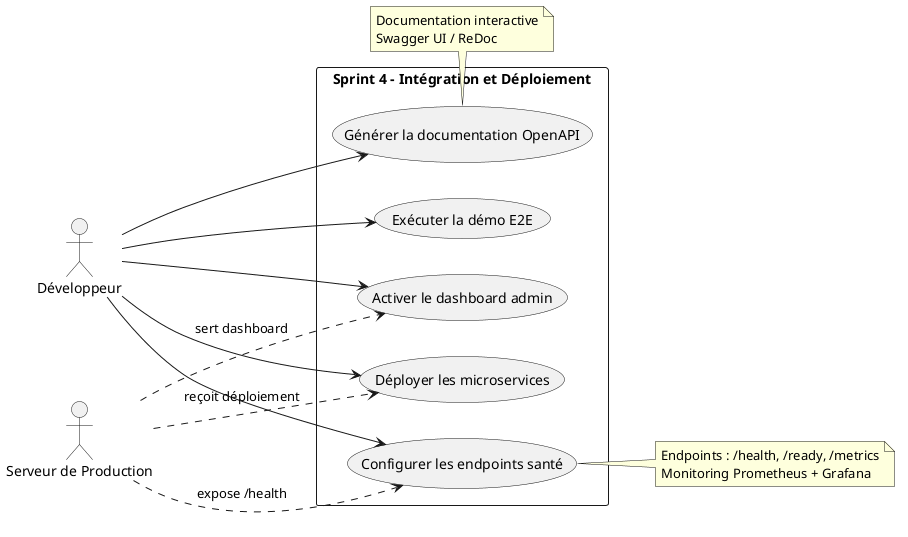
\includegraphics[width=0.85\textwidth]{diagrams/plantuml/usecase_sprint4.png}
    \caption{Diagramme de cas d'utilisation --- Sprint~4}
    \label{fig:uc_sprint4}
\end{figure}

\subsection{Description textuelle des cas d'utilisation}

\begin{table}[H]
    \centering
    \caption{Description textuelle --- CU : Obtenir des recommandations personnalisées}
    \label{tab:cu_sprint4_1}
    \small
    \begin{tabular}{p{3cm} p{10cm}}
        \toprule
        \textbf{Champ} & \textbf{Description} \\
        \midrule
        Titre & Obtenir des recommandations personnalisées \\[3pt]
        Acteur & Touriste / Système \\[3pt]
        Pré-condition & Des bras \texttt{BanditArm} existent pour la zone demandée \\[3pt]
        Scénario nominal &
        1. Le frontend envoie \texttt{GET /api/recommendations} avec paramètres de contexte \newline
        2. Les bras sont récupérés depuis le cache RAM \newline
        3. Le profil utilisateur est chargé si \texttt{user\_id} est fourni \newline
        4. Le vecteur $\phi$ est calculé par produit de Kronecker pour chaque bras \newline
        5. Le pipeline de classement en 10~étapes est exécuté \newline
        6. Les Top-K recommandations sont retournées \\[3pt]
        Post-condition & Un \texttt{RecommendationEvent} de type impression est enregistré \\
        \bottomrule
    \end{tabular}
\end{table}

\begin{table}[H]
    \centering
    \caption{Description textuelle --- CU : Tracker un événement comportemental}
    \label{tab:cu_sprint4_2}
    \small
    \begin{tabular}{p{3cm} p{10cm}}
        \toprule
        \textbf{Champ} & \textbf{Description} \\
        \midrule
        Titre & Tracker un événement comportemental \\[3pt]
        Acteur & Système (tracker JavaScript) \\[3pt]
        Pré-condition & Session active avec un \texttt{session\_id} valide \\[3pt]
        Scénario nominal &
        1. Le tracker JS détecte un événement (clic, scroll, favoris, réservation) \newline
        2. L'événement est mis en file d'attente \newline
        3. Flush toutes les 15~secondes ou tous les 10~événements \newline
        4. \texttt{POST /api/recommendations/events} envoie le lot \newline
        5. \texttt{compute\_reward()} calcule la récompense delta \newline
        6. Les matrices A et b sont mises à jour en RAM \\[3pt]
        Post-condition & Compteurs \texttt{BanditArm} et \texttt{RecommendationEvent} mis à jour \\
        \bottomrule
    \end{tabular}
\end{table}


% ────────────────────────────────────────────────────────────────
\section{Conception}
% ────────────────────────────────────────────────────────────────

\subsection{Diagramme de séquence --- Pipeline de recommandation}

\begin{figure}[H]
    \centering
    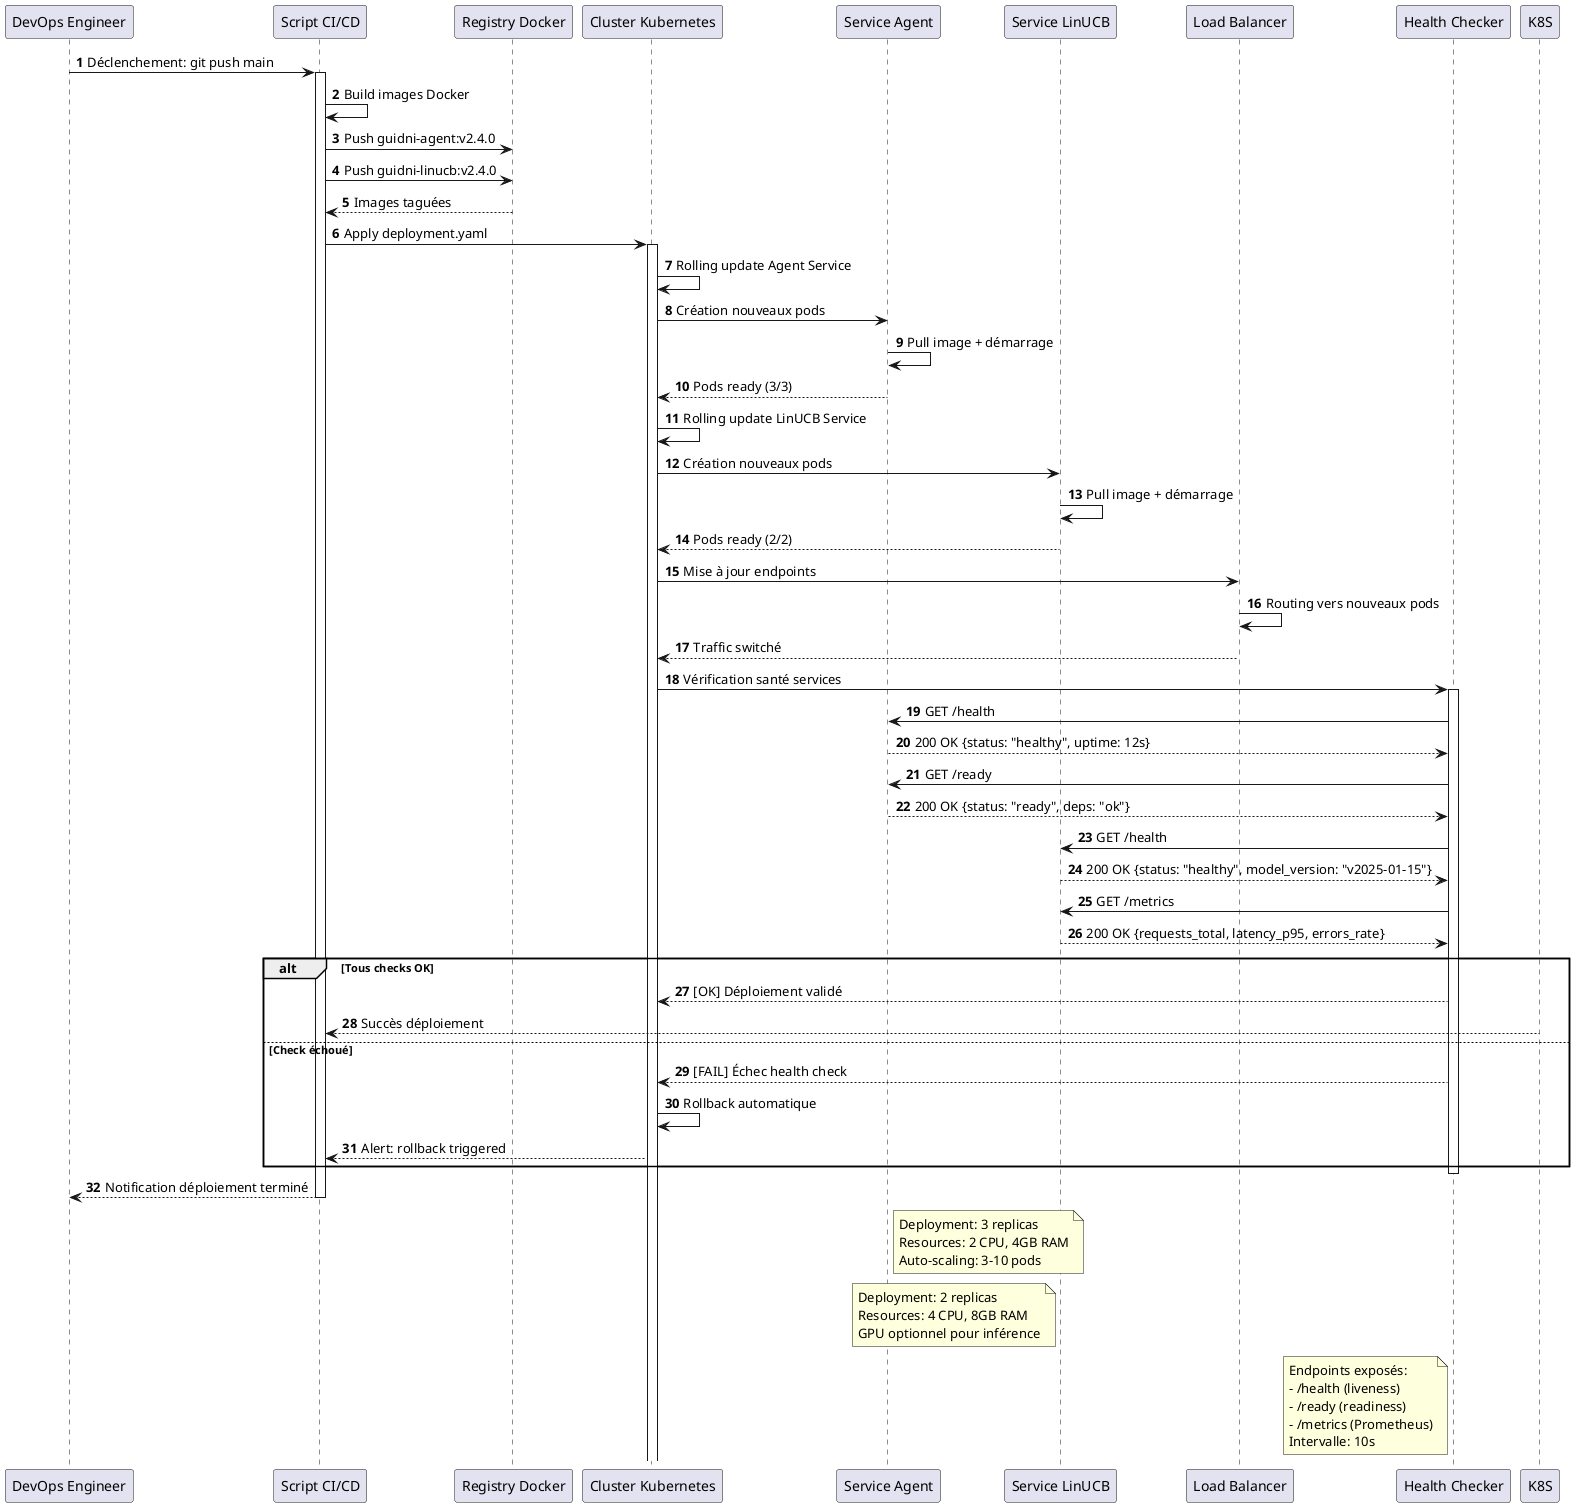
\includegraphics[width=\textwidth]{diagrams/plantuml/sequence_sprint4_primary.png}
    \caption{Diagramme de séquence --- Pipeline de recommandation LinUCB}
    \label{fig:seq_sprint4_primary}
\end{figure}

\subsection{Diagramme de séquence --- Traitement des événements comportementaux}

\begin{figure}[H]
    \centering
    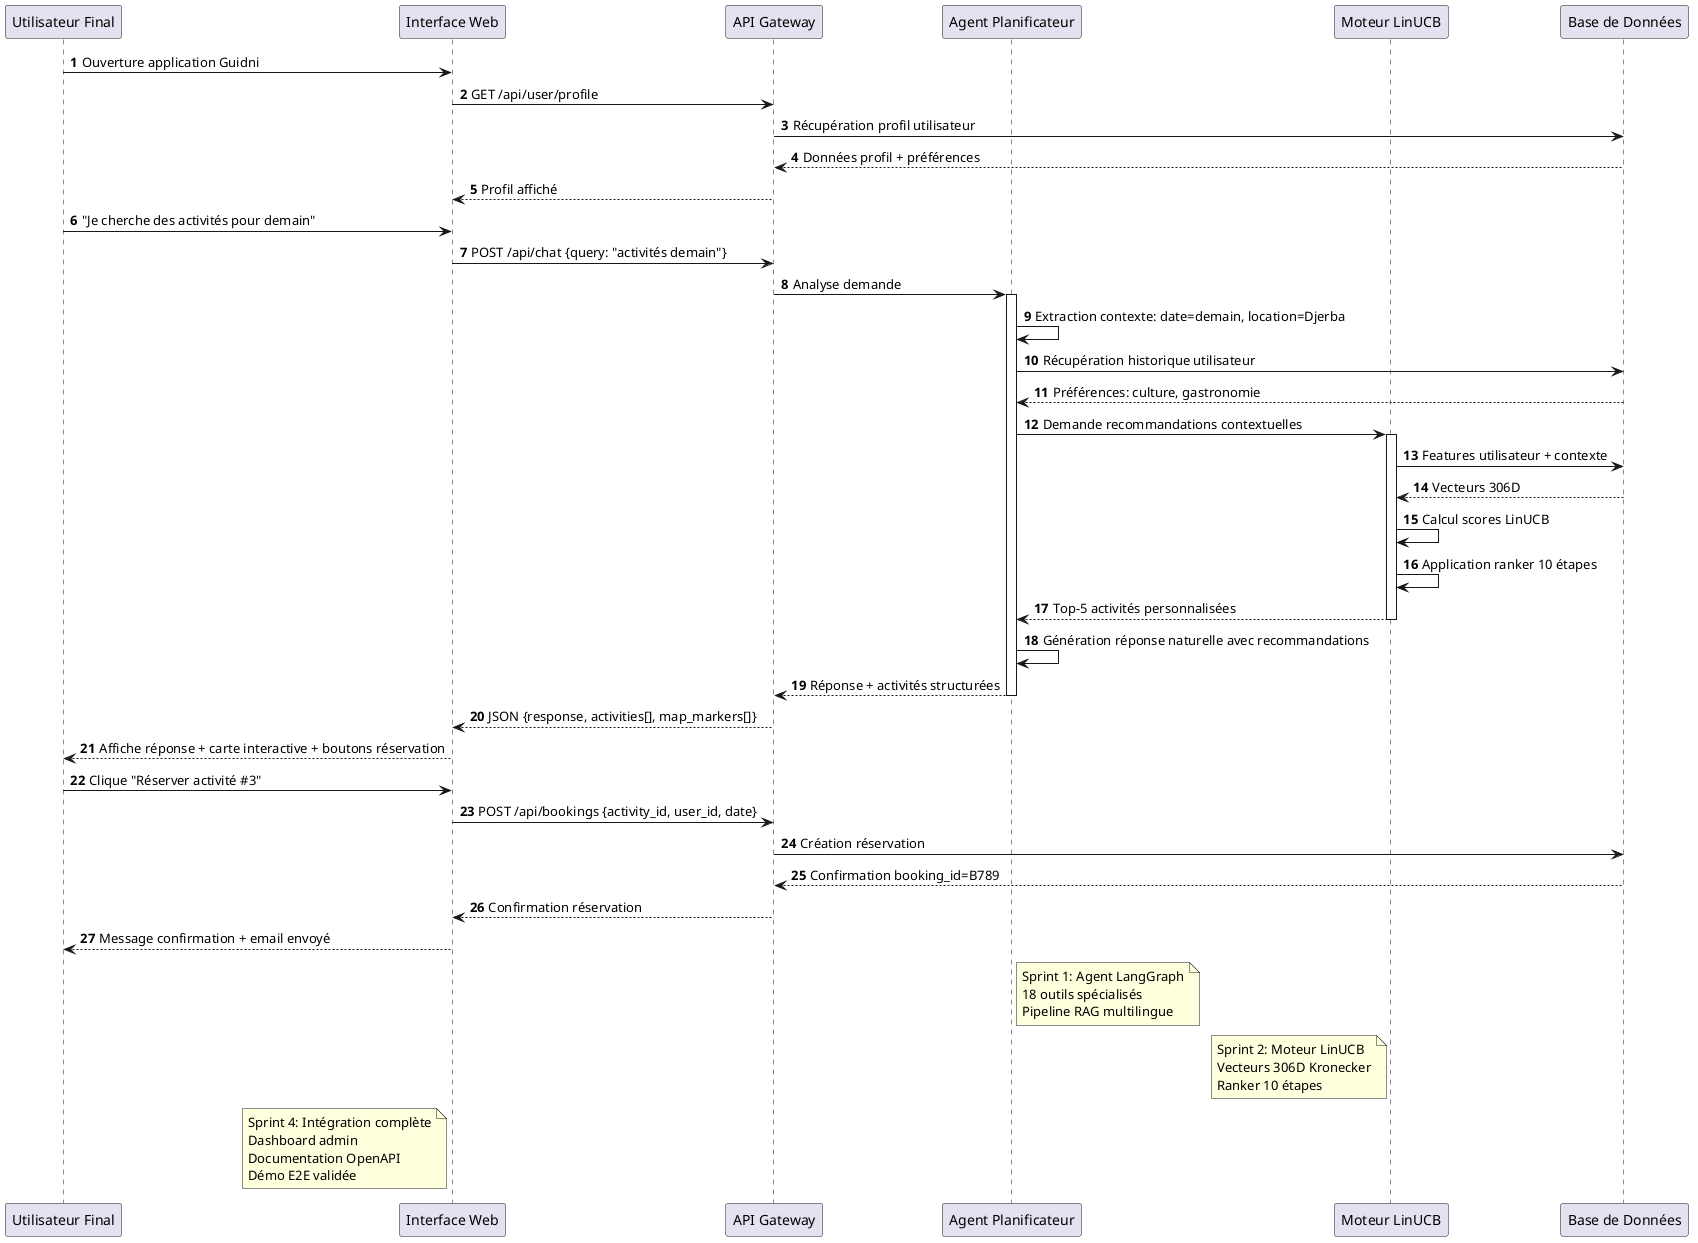
\includegraphics[width=\textwidth]{diagrams/plantuml/sequence_sprint4_secondary.png}
    \caption{Diagramme de séquence --- Traitement d'un lot d'événements comportementaux}
    \label{fig:seq_sprint4_secondary}
\end{figure}


% ────────────────────────────────────────────────────────────────
\section{Réalisation}
% ────────────────────────────────────────────────────────────────

\subsection{Processus du moteur LinUCB}

La figure suivante illustre le cycle d'exploitation/exploration du moteur LinUCB, depuis
la réception du contexte utilisateur jusqu'à la mise à jour des matrices suite à la
récompense observée.

\begin{figure}[H]
    \centering
    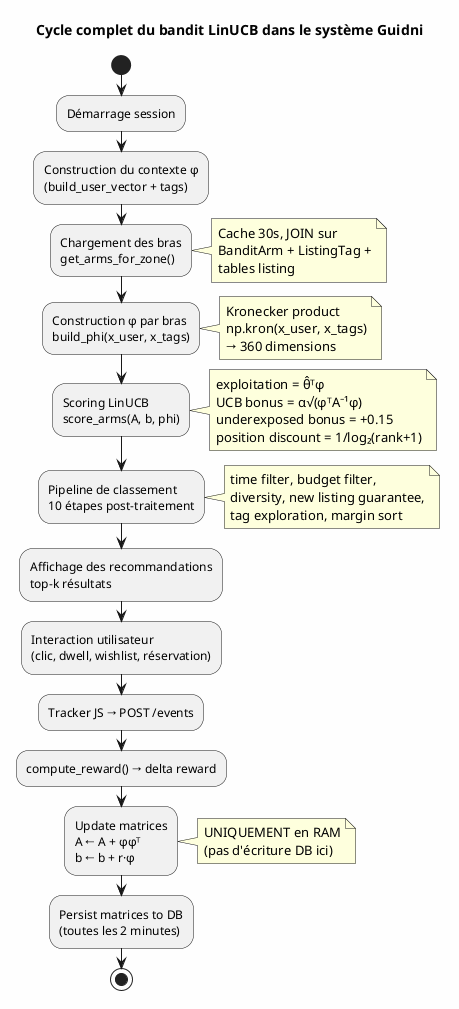
\includegraphics[width=0.75\textwidth]{diagrams/fig_02_linucb_cycle.png}
    \caption{Processus du moteur LinUCB --- cycle exploitation/exploration}
    \label{fig:linucb_process}
\end{figure}

\subsection{Moteur de scoring LinUCB}

Le moteur LinUCB a été implémenté avec les composants suivants~:

\begin{itemize}
    \item \textbf{Vecteur de caractéristiques} $\phi$ de dimension~306, construit par produit
    de Kronecker~: $\phi = x_{\text{user}}(9) \otimes x_{\text{tags}}(34)$.
    \item \textbf{Matrice globale} $A$ ($306 \times 306$) et vecteur cible $b$ ($306$),
    partagés entre toutes les annonces dans \texttt{LinUCBGlobal}.
    \item \textbf{Cache en RAM} avec verrou \texttt{threading.Lock} pour un accès quasi
    instantané, avec persistance asynchrone en base toutes les 2~minutes via APScheduler.
    \item \textbf{Score UCB}~: $\text{score} = \hat{\theta}^\top \phi + \alpha
    \sqrt{\phi^\top A^{-1} \phi}$ avec $\alpha = 0.3$.
\end{itemize}

\begin{table}[H]
    \centering
    \caption{Les 9 composantes du vecteur utilisateur $x_{\text{user}}$}
    \label{tab:user_vector}
    \small
    \begin{tabular}{c l l}
        \toprule
        \textbf{Idx} & \textbf{Caractéristique} & \textbf{Formule} \\
        \midrule
        0 & sin(heure) & $\sin(2\pi \times h / 24)$ \\
        1 & cos(heure) & $\cos(2\pi \times h / 24)$ \\
        2 & sin(mois) & $\sin(2\pi \times m / 12)$ \\
        3 & cos(mois) & $\cos(2\pi \times m / 12)$ \\
        4 & Profondeur défilement & $\text{clip}(\text{scroll}, 0, 1)$ \\
        5 & Temps consultation & $\text{clip}(\log(1+\text{dwell})/\log(301), 0, 1)$ \\
        6 & Affinité prix & $\text{avg\_price} / 2000$ \\
        7 & Affinité tag max & $\max(\text{tag\_affinity})$ \\
        8 & Type voyage & famille$=1.0$, couple$=0.67$, solo$=0.33$ \\
        \bottomrule
    \end{tabular}
\end{table}

\subsection{Pipeline de classement en 10 étapes}

Le fichier \texttt{ranker.py} déploie un pipeline séquentiel en dix étapes~:
\begin{enumerate}
    \item Correction de popularité (bonus +0.15 si $<$50 impressions)
    \item Filtre temporel (pas de bar le matin, pas d'activité matinale le soir)
    \item Filtre budgétaire (prix $\leq$ budget $\times$ 1.25)
    \item Construction des vecteurs $\phi$ (produit de Kronecker)
    \item Scoring LinUCB (formule UCB)
    \item Filtre de diversité (max 2 annonces par type)
    \item Garantie nouvelles annonces (1 sous-exposée minimum)
    \item Exploration de tags (10\% de tags non explorés)
    \item Tri par marge (commission pour les ex-æquo)
    \item Extraction Top-K (10 par défaut)
\end{enumerate}

\begin{figure}[H]
    \centering
    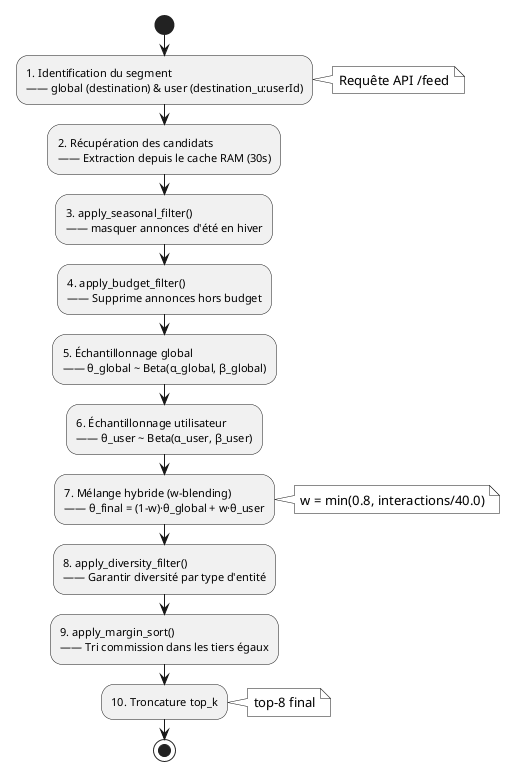
\includegraphics[width=0.85\textwidth]{diagrams/fig_05_ranker_pipeline.png}
    \caption{Organigramme du pipeline de classement en 10 étapes}
    \label{fig:ranker_pipeline}
\end{figure}

\subsection{Tracker comportemental JavaScript}

Le tracker JavaScript vanilla, sans dépendance externe, analyse le navigateur du client et
collecte huit types de signaux avec des valeurs de récompense prédéfinies~:

\begin{table}[H]
    \centering
    \caption{Signaux de récompense du tracker comportemental}
    \label{tab:rewards}
    \small
    \begin{tabular}{l c l}
        \toprule
        \textbf{Signal} & \textbf{Récompense} & \textbf{Description} \\
        \midrule
        quick\_exit & $-0.2$ & Sortie en $<$5 secondes \\
        impression & $0.0$ & Simple affichage \\
        click & $0.3$ & Clic sur l'annonce \\
        gallery\_swipe & $0.4$ & Balayage de la galerie \\
        dwell\_30s & $0.5$ & Consultation $\geq$30 secondes \\
        scroll\_reviews & $0.6$ & Lecture des avis \\
        dwell\_60s & $0.7$ & Consultation $\geq$60 secondes \\
        wishlist & $0.85$ & Ajout aux favoris \\
        reservation & $1.0$ & Réservation ferme \\
        \bottomrule
    \end{tabular}
\end{table}

\begin{figure}[H]
    \centering
    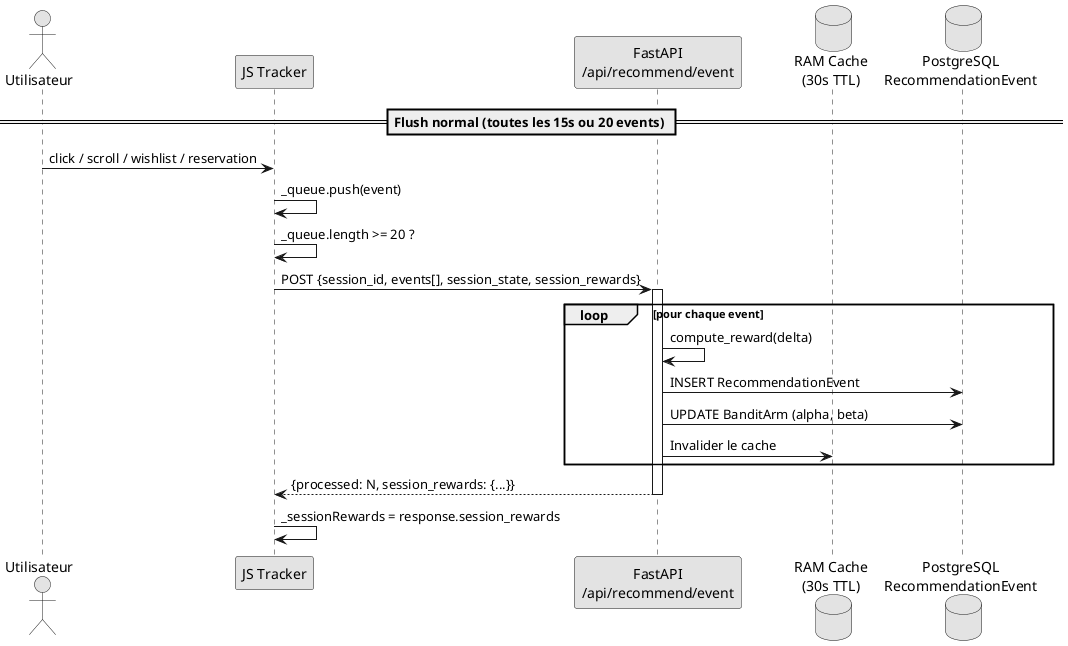
\includegraphics[width=0.85\textwidth]{diagrams/fig_05_tracker_flush.png}
    \caption{Flux du tracker JavaScript --- mise en file d'attente et flush par lot}
    \label{fig:tracker_flush}
\end{figure}

\subsection{Stratégie de tests}

La stratégie de tests stratifiée, orchestrée par \texttt{pytest}, comprend trois couches~:
\begin{itemize}
    \item \textbf{Tests unitaires}~: chaque fonction pure (normalisation des vecteurs $\phi$,
    filtrage budgétaire, calcul de score) testée par assertion.
    \item \textbf{Tests d'intégration}~: fluidité des interactions entre composants et
    persistance relationnelle (Event Loop FastAPI sans blocage).
    \item \textbf{Tests système}~: orchestration end-to-end de l'agent LangGraph avec les
    18~outils.
\end{itemize}

\subsection{Évaluation du pipeline RAG}

L'évaluation quantitative repose sur l'injection de 20~requêtes test couvrant le spectre
trilingue (FR/EN/AR) avec des critères discriminants~: contraintes géographiques, notions
subjectives (romantisme, adrénaline) et limitations budgétaires. Les résultats attestent
d'une préservation sémantique élevée (Precision@K) justifiant l'hybridation multilingue.

\subsection{Simulation du moteur LinUCB}

Un banc d'essai émulant 500~sessions d'exploration avec des comportements de clics orientés
a été programmé. Le cumul de la récompense (Cumulative Reward) croît significativement au fil
des itérations, supplantant une stratégie aléatoire et démontrant le franchissement de la
phase de Cold Start.

\begin{figure}[H]
    \centering
    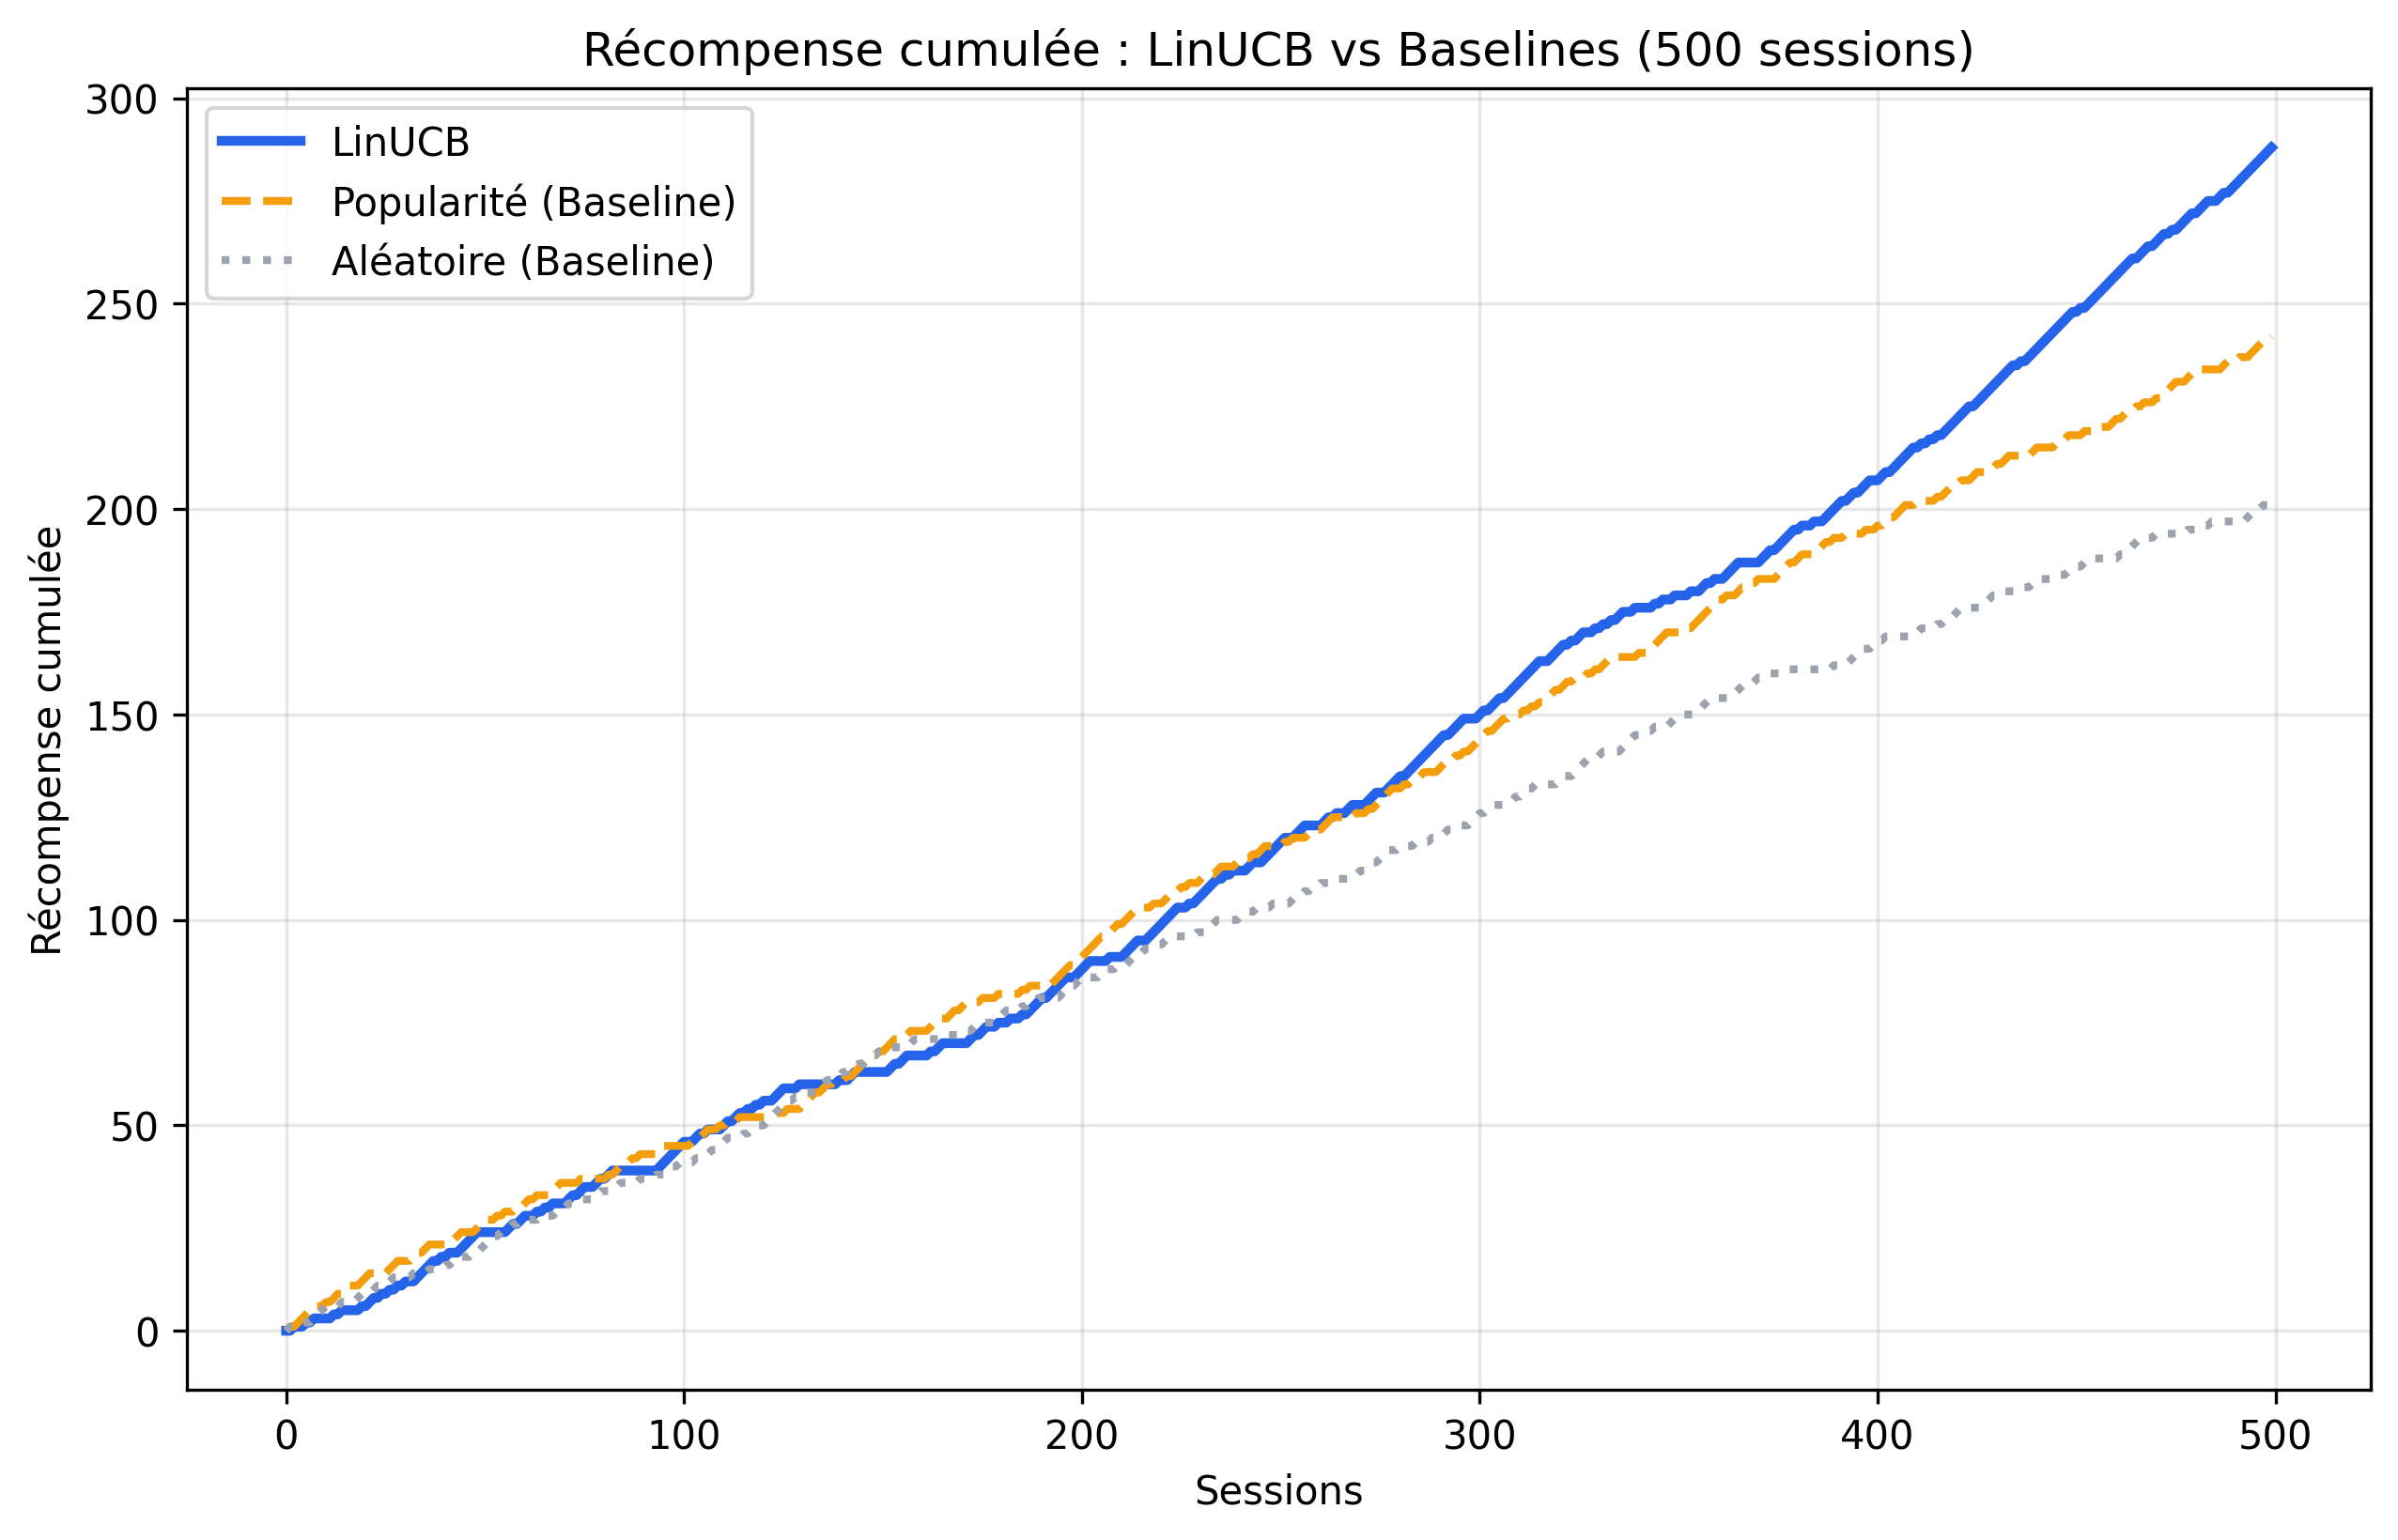
\includegraphics[width=0.85\textwidth]{diagrams/fig_06_cumulative_reward.png}
    \caption{Résultats de la simulation LinUCB (500 sessions)}
    \label{fig:linucb_simulation}
\end{figure}

\subsection{Recommandations affichées}

\begin{figure}[H]
    \centering
    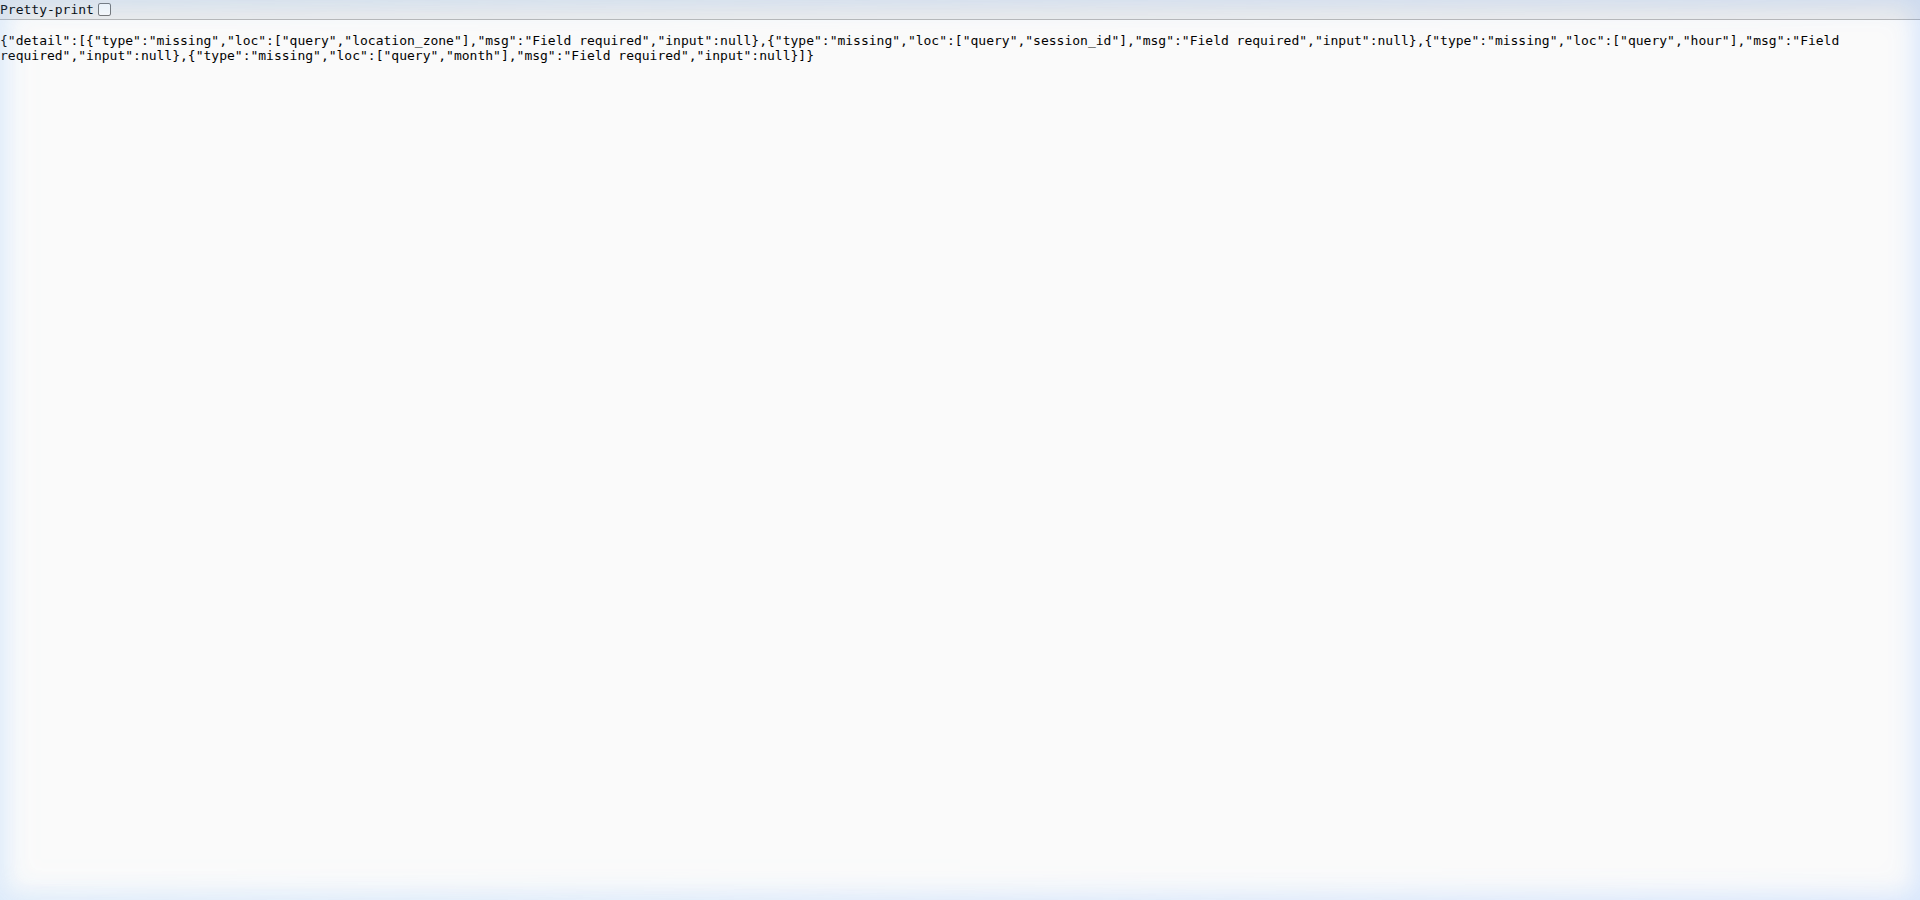
\includegraphics[width=\textwidth]{diagrams/screen_A4_recommendations_response.png}
    \caption{Recommandations personnalisées affichées sur la plateforme}
    \label{fig:screen_reco}
\end{figure}

\subsection{Supervision du système}

\begin{figure}[H]
    \centering
    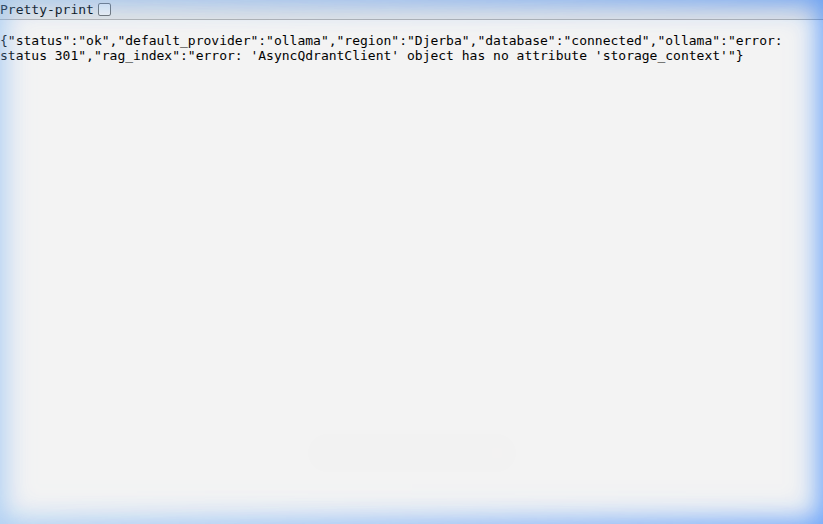
\includegraphics[width=\textwidth]{diagrams/screen_06_health_endpoint.png}
    \caption{Endpoint de santé du système avec statut des composants}
    \label{fig:screen_health_sprint4}
\end{figure}


% ────────────────────────────────────────────────────────────────
\section{Sprint Review}
% ────────────────────────────────────────────────────────────────

Lors de la Sprint Review finale, Guidni a été mis à l'essai dans un scénario continu simulant
une visite prolongée~: le raisonneur conversationnel combiné à l'affichage instantané des
recommandations LinUCB. L'ingestion de cent événements comportementaux via Postman a abouti
à une rotation des recommandations en faveur de séjours maritimes. La contrainte de latence
sous les 100~ms a été démontrée conforme, les chronomètres validant des inférences oscillant
entre 5 et 10~ms en condition locale.

L'encadrant a reconnu la satisfaction intégrale des prérequis fonctionnels et qualitatifs
du PFE. La Sprint Retrospective globale a consolidé un retour d'expérience édifiant sur
l'importance de l'organisation Scrum pour les systèmes d'IA évolutifs.


% ────────────────────────────────────────────────────────────────
\section*{Conclusion}
\addcontentsline{toc}{section}{Conclusion}

Le Sprint~4 a finalisé le développement du système Guidni par l'implémentation du moteur
de recommandation LinUCB avec son pipeline en 10~étapes, le tracker JavaScript, les jobs
nocturnes et les campagnes de tests et d'évaluation. Les simulations ont confirmé la
convergence prédictive du modèle et la satisfaction des contraintes de latence. Ce Sprint
conclut le cycle de développement itératif Scrum du projet Guidni. Le chapitre suivant
présentera la conclusion générale et les perspectives d'évolution future.
